\section{Planteamiento del problema}
	La  integración  sensorial  es  un  área  fundamental  en  terapia  ocupacional  la cual trabaja  todo  lo  referente  a  la  parte  sensorio-motora  especialmente  en  niños  de diferentes edades,  esto  permite  observar  el  comportamiento de  los  niños  a  cierta edad,  por  ejemplo  según  las  etapas  de  desarrollo  normal  de  un  niño,  la  edad adecuada para aprender a anudarse los zapatos es a los 6 años pero en ocasiones algunos niños se les dificulta y pueden tardarse más tiempo en aprender, este es un síntoma para percibir que el niño tiene retrasos en su desarrollo por lo cual es necesario la asistencia de especialistas en terapia ocupacional que le den base a los niños para aprender a realizar esta labor por sus propios medios, así mismo se presentan  problemas  con  diferentes  actividades  que  en  algún  momento  deberían aprender y que son base para su desarrollo además de que les servirá para el resto de sus vidas.\\
	Cuando un terapeuta realiza la valoración de su paciente debe realizar una serie de actividades  donde  recree  diferentes  etapas  las  cuales dan  un  diagnóstico  de  que problemática o retraso puede estar presentando un niño, con esto genera una base para realizar una serie de tratamientos que ayudarían en el proceso de desarrollo de los niños, la problemática se encuentra en que estos son procesos largos para un profesional ya que existen muchas formas de tratar los retrasos a su vez se debe tener  en  cuenta  que  estos  deben  ser  dinámicos  para  que  los  niños  no  entren  en aburrimiento con los tratamientos que se aplican, a su vez los tiempos para generar un diagnostico claro pueden llevar hasta dos o tres semanas tiempo en que el niño puede aprovecharlo para avanzar en un tratamiento.\\
	Para  dar  una  solución  a  la  problemática  mencionada  se  requiere  un  prototipo  de software en el cual se pueda realizar el registro del diagnóstico y este a través de redes  neuronales pueda  generar  sugerencias  para  el  tratamiento  de  los  niños reduciendo  los  tiempos  que  este  le  tomaba  a  los  terapeutas  que  realizaban  el proceso de valoración.
	\subsection{Formulación del problema}
		¿Cómo  se  debe  sistematizar  el  proceso  a  través  de redes  neuronales  para modelado de sistemas dinámicos el cual permita realizar diagnósticos y encontrar posibles tratamientos para el desarrollo de niños con problemas vestibulares?\\
	\subsection{Sistematización del problema}
		\begin{itemize}
			\item ¿Cómo crear un sistema el cual pueda dar un diagnostico real y acertado en niño a través de redes neuronales?.
			\item ¿Cómo crear y contar con variedad de tratamientos y cuál sería la manera factible de categorizarlos para que se adecuen según el problema vestibular que tenga un niño?
			\item ¿Cuál es el impacto de los resultados obtenidos en tratamientos generados a través del  aplicativo  y  que  beneficios  da  con  respecto  a  tratamientos creados de forma manual?.
		\end{itemize}
\newpage
\section{Objetivos de la investigación}
	\subsection{Objetivo General}
	Desarrollar prototipo de software para la evaluación y diagnosticó de niños con problemas vestibulares utilizando redes neuronales para el modelado de sistemas dinámicos.
	\subsection{Objetivos Específicos}
	\begin{itemize}
		\item Elaborar un sistema de diagnóstico para identificar los posibles problemas vestibulares que tiene un niño al ser valorado.
		\item Elaborar un sistema de tratamientos los cuales sean adecuados para tratar un problema vestibular en los niños y ver su evolución
		\item Elaborar comparativas entre los tratamientos generados y tratamientos establecidos de manera manual para ver la evolución de los niños y cual ha servido de manera más efectiva.
	\end{itemize}
\newpage
\section{Justificación de la investigación}
	\subsection{Justificación teórica}
		El vértigo y los trastornos del equilibrio son patologías que en algún momento de la etapa de crecimiento puede afectar a un niño y la cual pueden a su vez estar presentes para toda la vida, es por esto por lo que cuando un niño se marea fácilmente cuando se viaja en carro o en otro medio de transporte es necesario tratarlo para darle un mejor desarrollo a su sistema vestibular y que a futuro pueda tener mejor calidad de vida.\\
		De allí se obtiene que la presente investigación tenga como objeto de estudio el uso de redes neuronales para crear alternativas de tratamiento en los niños que pueda dar una alternativa en la búsqueda de estas ya que no convierte los tratamientos en algo limitado, sino que expande la noción y el uso que le pueda dar un terapeuta en pro del beneficio del niño en sus etapas de desarrollo.\\
\section{Hipótesis de trabajo}
	Desarrollar el prototipo permitirá optimizar y realizar una mejor labor al momento de atender a niños con problemas vestibulares dando más alternativas de tratamientos que ayudaran al terapeuta a tratar los problemas que tenga y al final se puede ver la mejora generada por los tratamientos ejecutados ya que el aplicativo tendrá la capacidad de buscar la mejor alternativa para un tratamiento efectivo.\\
\section{Marco referencial}
	\subsection{Marco Teórico}
		\subsubsection{Teoría de Integración Sensorial:}
			La Dra. Jean Ayres, (1972) fue una de las precursoras de la teoría de IS, quien logra explicar la íntima relación que existe entre el sistema nervioso y la conducta, puesto que, el proceso de IS es soberanamente adaptativo y entrelaza información proveniente de diferentes canales sensoriales para descubrir mejor, reconocer y reaccionar a los acontecimientos del ambiente, de ahí que, la IS es crítica para la percepción y la conducta. \\
			De acuerdo con lo anterior, se establecen cinco (5) posturas que aportan a la relación entre el sistema nervioso y la conducta:
			\begin{itemize}
				\item La reacción del sistema nervioso ante las situaciones de las que es participe el ser humano, se le conoce como neuroplasticidad.
				\item El cerebro actúa como un conjunto jerárquico integrado por niveles superiores que adquieren el control y son controlados por las funciónes proporcionadas a cada nivel.
				Existe una secuencia evolutiva que da como resultado la interacción entre maduración cerebral y acumulación de experiencias sensoriales.
				\item La disposición del cerebro y la conducta adaptativa son interactivas.
				\item Los individuos conservan impulso interno para cumplir retos en actividades sensoriales motoras.
			\end{itemize}
			El desarrollo de integración sensorial se considera como un aspecto de carácter automático e inconsciente que permite entender el continuo del procesamiento sensorial. El cual tiene como objetivo entender el funciónamiento del procesamiento cerebral desde el inicio: entrada-integración-salida / entorno-cerebro-conducta. \\
			Ayres, crea el siguiente esquema para mostrar que las sensaciones son la entrada primaria de información, para luego convertirse en una representación corporal que a su vez da respuesta a una actividad con un propósito especifico; lo cual favorece la constitución de funciónes integrales en el cerebro y finalmente una especialización natural de los dos lados del cuerpo y del cerebro. Todo lo anterior con el fin de precisar un aprendizaje significativo entre el sentido y la interacción con el medio.\\
			\begin{figure}
				\centering
				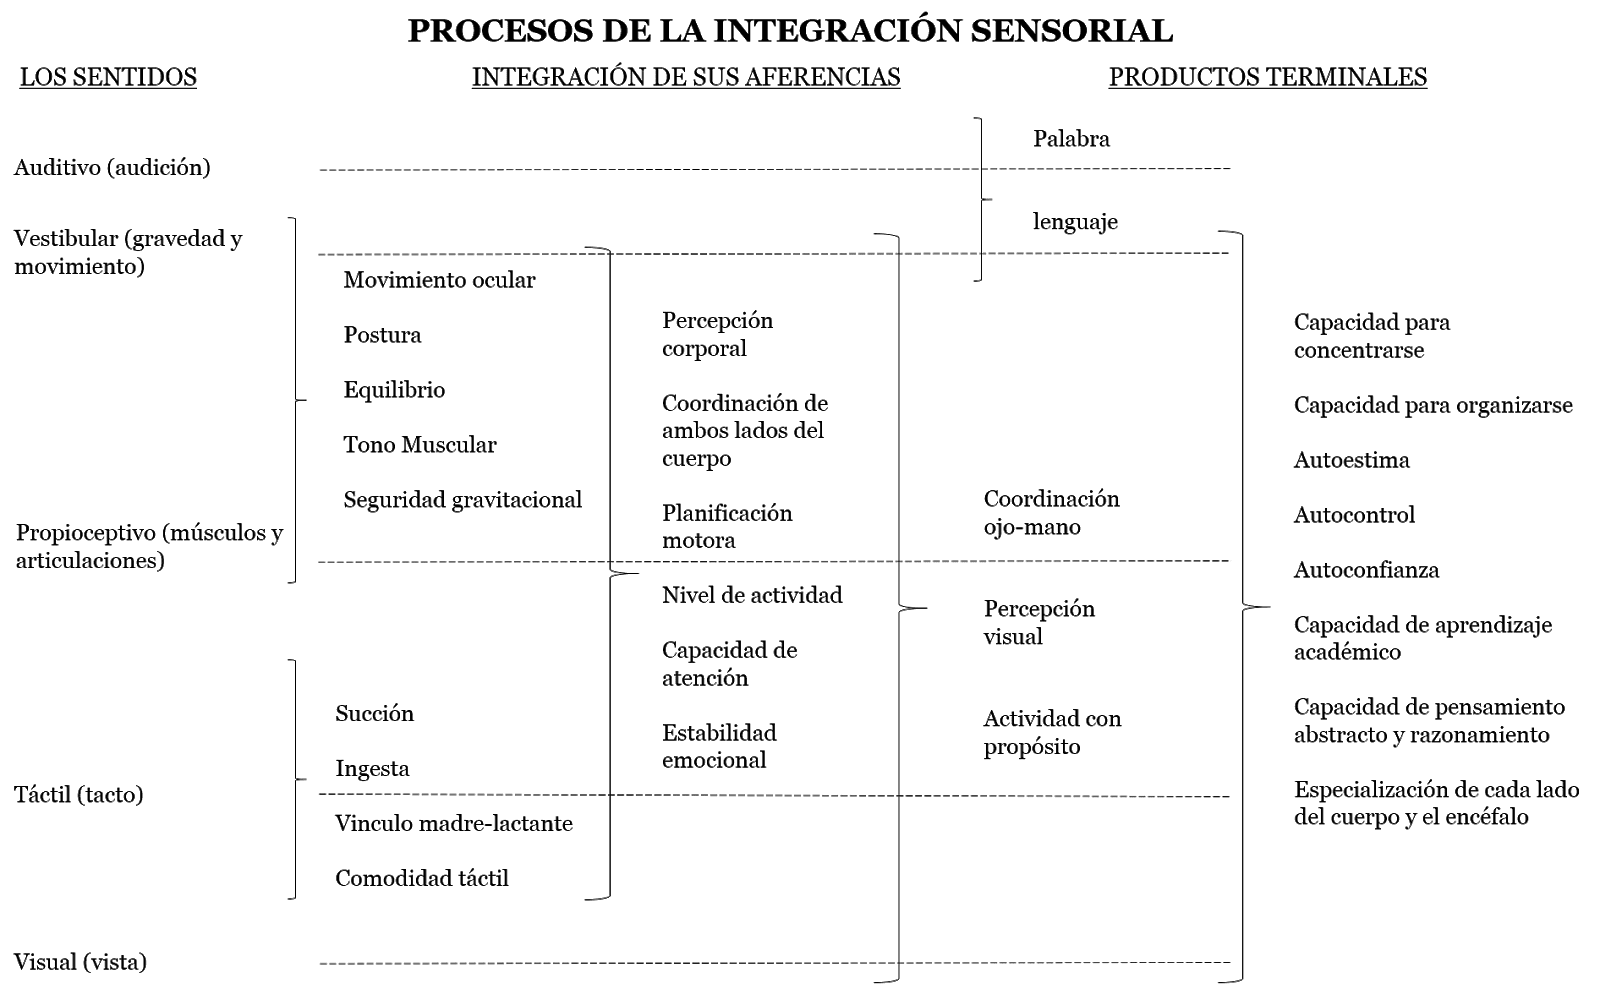
\includegraphics[width=10cm]{Imagenes/Figuras/01.png}
				\caption{Los sentidos, integración de sus entradas y su producto fina}
			\end{figure}
			Alteraciones o problemas del desarrollo
			Cuando se hace referencia a desarrollo psicomotor normal se habla de un proceso que permite al niño adquirir habilidades adecuadas para su edad. No obstante, como se mencionó, existe gran variabilidad en la edad en la adquisición o alcance de diferentes habilidades. Esto es relevante porque da cuenta de la dificultad de establecer claramente un límite entre lo "normal" y lo "patológico". En general, ambas esferas son diferenciadas con criterios de normalidad estadística bajo los términos desvío, significación y promedio. Así Poo Argüelles planteó “Que lo patológico es apartarse de una manera significativa de lo esperado para la edad, en un área concreta o en la globalidad e Illingworth sostuvo lo único que se puede decir es que cuanto más lejos del promedio se encuentre un niño, en cualquier aspecto, es menos probable que sea normal”. En esta perspectiva, cuando el DPM presenta características peculiares o diferentes a la "norma", se está en presencia de alteraciones o problemas del desarrollo. ¿Pero cuán apartado de la norma debe estar el DPM para ser considerado patológico? En general es sencillo estar de acuerdo en lo "muy patológico", pero no tanto cuando se intentan definir ciertas alteraciones o trastornos, que pueden discurrir entre ambos extremos.\\
			El DPM puede presentar variantes o alteraciones diversas. El retraso psicomotor, los diferentes tipos de trastornos del desarrollo y los problemas inaparentes del desarrollo son ejemplos de este tipo de alteraciones. El retraso psicomotor es uno de los cuadros más frecuentemente detectados en niños pequeños. Narbona y Schlumberger lo definieron como “un diagnóstico provisional, en donde los logros del desarrollo de un determinado niño durante sus primeros tres años de vida aparecen con una secuencia lenta para su edad y/o cualitativamente alterada”. El término retraso psicomotor, entonces, se suele mantener hasta que pueda establecerse un diagnóstico definitivo a través de pruebas formales (Accardoy otros, 2001). Alvarez Gómez et al sostienen que “debido a que es un término muy indefinido, no debería utilizarse más allá de los tres a cinco años de edad del niño, cuando ya se pueden realizar tests que miden la capacidad intelectual”.\\
			En España el término retraso psicomotor se utiliza como sinónimo de retraso del desarrollo, mientras que en América Latina es más frecuente el término retraso madurativo. Álvarez Gómez et al, por otra parte, definen al retraso del desarrollo como una demora o lentitud en la secuencia normal de adquisición de los hitos del desarrollo, por lo cual para estos autores no existe nada intrínsecamente anormal, los hitos madurativos se cumplen en el orden esperado, sólo que en forma más lenta. Esto implica que, a largo plazo, el niño adquirirá las habilidades deficitarias y siempre seguirá un orden específico en la adquisición de estas.
			Por lo anteriormente mencionado, el niño con retrasos en su desarrollo puede normalizarse a largo plazo y, cuando esto no ocurre, será diagnosticado con una cierta patología. Narbona y Schlumberger “contemplaron las diferentes posibilidades diagnósticas en las que puede desembocar un cuadro que inicialmente se manifestó como un retraso psicomotor de la siguiente manera: puede ocurrir que el retraso sea una variante normal del desarrollo, en cuyo caso se normalizará espontáneamente antes de la edad preescolar”. Puede que en realidad sea un verdadero retraso, debido a déficit en la estimulación por parte del entorno familiar y social, que podría ser normalizado si se adecuara la educación y el ambiente del niño (retraso de etiología ambiental); o bien deberse a enfermedad crónica extraneurológica (cardiopatía congénita, enfermedad respiratoria, desnutrición, entre otras), compensándose en la medida en que mejora la enfermedad general de base. Por otra parte, un retraso puede deberse al efecto de un déficit sensorial aislado, como la sordera neurosensorial congénita o ser la primera manifestación de una futura deficiencia mental, cuyo diagnóstico definitivo en los casos leves, no suele evidenciarse hasta el final de la edad preescolar. Otra posibilidad es que sea la primera manifestación de una encefalopatía crónica no evolutiva, un trastorno neuromuscular congénito de escasa o nula evolutividad, la primera manifestación de una futura torpeza selectiva en la psicomotricidad fina y/o gruesa (trastorno del desarrollo de la coordinación, frecuentemente asociado a la forma disatencional del TDAH), o el inicio de un trastorno global del desarrollo (trastorno de tipo autista).\\
			A veces es relativamente sencillo percibir si el retraso puede ser transitorio o no. En los casos en que los retrasos están asociados a otros signos o características físicas o dismorfias, por ejemplo, es más frecuente que se trate de un cuadro que tienda a mantenerse en el tiempo. Lo mismo ocurre en el retraso global del desarrollo donde hay alteración de dos o más áreas o campos del desarrollo, manifestándose un retraso significativo, correspondiente a dos o más desviaciones estándar inferior a la media en pruebas acorde a la edad del niño. Algunos ejemplos de trastornos globales del desarrollo son el autismo, el síndrome de Asperger o el síndrome de Rett. Cuando el problema del desarrollo es leve o sutil, puede no ser fácilmente evidenciable y para detectarlo es necesario realizar una prueba de pesquisa o screening. En estos casos podría hablarse de trastornos inaparentes del desarrollo psicomotor. Dado que la mayoría de los lactantes y preescolares con dificultades del desarrollo no tienen signos obvios de enfermedad, por lo menos en un inicio, ni factores de riesgo que lo sugieran, la identificación de estos niños aparentemente sanos suele constituir un verdadero desafío. Los trastornos inaparentes del desarrollo plantean tal vez la discusión más difícil en esta área y transcurren en un límite difuso entre lo "normal y patológico".\\
	\subsection{Marco Conceptual}
		Interfaz de usuario: La interfaz de usuario es el medio con que el usuario puede comunicarse con una máquina, un equipo o una computadora, y comprende todos los puntos de contacto entre el usuario y el equipo. Normalmente suelen ser fáciles de entender y fáciles de accionar. Las interfaces básicas de usuario son aquellas que incluyen elementos como menús, ventanas, teclado, ratón, los beeps y algunos otros sonidos que la computadora hace, y en general, todos aquellos canales por los cuales se permite la comunicación entre el ser humano y la computadora. La mejor interacción humano-máquina a través de una adecuada interfaz (Interfaz de Usuario), que le brinde tanto comodidad, como eficiencia.
		Tipos de interfaces de usuario: Dentro de las Interfaces de Usuario se puede distinguir básicamente tres tipos:
		Una interfaz de hardware, a nivel de los dispositivos utilizados para ingresar, procesar y entregar los datos: teclado, ratón y pantalla visualizadora.
		Una interfaz de software, destinada a entregar información acerca de los procesos y herramientas de control, a través de lo que el usuario observa habitualmente en la pantalla.
		Una interfaz de Software-Hardware, que establece un puente entre la máquina y las personas, permite a la máquina entender la instrucción y a el hombre entender el código binario traducido a información legible.
		Funciones principales: Sus principales funciones son las siguientes:
		Puesta en marcha y apagado.
		Control de las funciones manipulables del equipo.
		Manipulación de archivos y directorios.
		Herramientas de desarrollo de aplicaciones.
		Comunicación con otros sistemas.
		Información de estado.
		Configuración de la propia interfaz y entorno.
		Intercambio de datos entre aplicaciones.
		Control de acceso.
		Sistema de ayuda interactivo.
		Tipos de interfaces de usuario
		Según la forma de interactuar del usuario
		Atendiendo a como el usuario puede interactuar con una interfaz, nos encontramos con varios tipos de interfaces de usuario:
		Interfaces alfanuméricas (intérpretes de comandos) que solo presentan texto.
		Interfaces gráficas de usuario (GUI, graphic user interfaces), las que permiten comunicarse con el ordenador de una forma muy rápida e intuitiva a representando gráficamente los elementos de control y medida.
		Interfaces táctiles, que representan gráficamente un "panel de control" en una pantalla sensible que permite interactuar con el dedo de forma similar a si se accionara un control físico.
		Según su construcción Pueden ser de hardware o de software:
		Interfaces de hardware: Se trata de un conjunto de controles o dispositivos que permiten que el usuario intercambie datos con la máquina, ya sea introduciéndolos (pulsadores, botones, teclas, reguladores, palancas, manivelas, perillas) o leyéndolos (pantallas, diales, medidores, marcadores, instrumentos).
		Interfaces de software: Son programas o parte de ellos, que permiten expresar nuestros deseos al ordenador o visualizar su respuesta.
		Redes Neuronales: “Las redes neuronales también conocidas como sistemas conexionistas son un modelo computacional basado en un gran conjunto de unidades neuronales simples (neuronas artificiales) de forma aproximadamente análoga al comportamiento observado en los axones de las neuronas en los cerebros biológicos. La información de entrada atraviesa la red neuronal (donde se somete a diversas operaciones) produciendo unos valores de salida.
		Cada neurona está conectada con otras a través de unos enlaces. En estos enlaces el valor de salida de la neurona anterior es multiplicado por un valor de peso. Estos pesos en los enlaces pueden incrementar o inhibir el estado de activación de las neuronas adyacentes. Del mismo modo, a la salida de la neurona, puede existir una función limitadora o umbral, que modifica el valor resultado o impone un límite que se debe sobrepasar antes de propagarse a otra neurona. Esta función se conoce como función de activación.
		Estos sistemas aprenden y se forman a sí mismos, en lugar de ser programados de forma explícita, y sobresalen en áreas donde la detección de soluciones o características es difícil de expresar con la programación convencional. Para realizar este aprendizaje automático, normalmente, se intenta minimizar una función de pérdida que evalúa la red en su total. Los valores de los pesos de las neuronas se van actualizando buscando reducir el valor de la función de pérdida. Este proceso se realiza mediante la propagación hacia atrás.
		El objetivo de la red neuronal es resolver los problemas de la misma manera que el cerebro humano, aunque las redes neuronales son más abstractas. Los proyectos de redes neuronales modernos suelen trabajar desde unos miles a unos pocos millones de unidades neuronales y millones de conexiones que, si bien son muchas órdenes, siguen siendo de una magnitud menos compleja que la del cerebro humano, más bien cercana a la potencia de cálculo de un gusano.
		Nuevas investigaciones sobre el cerebro a menudo estimulan la creación de nuevos patrones en las redes neuronales. Un nuevo enfoque está utilizando conexiones que se extienden mucho más allá y capas de procesamiento de enlace en lugar de estar siempre localizado en las neuronas adyacentes. Otra investigación está estudiando los diferentes tipos de señal en el tiempo que los axones se propagan, como el aprendizaje profundo, interpola una mayor complejidad que un conjunto de variables booleanas que son simplemente encendido o apagado.
		Las redes neuronales se han utilizado para resolver una amplia variedad de tareas, como la visión por computador y el reconocimiento de voz, que son difíciles de resolver usando la ordinaria programación basado en reglas. Históricamente, el uso de modelos de redes neuronales marcó un cambio de dirección a finales de los años ochenta de alto nivel, que se caracteriza por sistemas expertos con conocimiento incorporado en si-entonces las reglas, a bajo nivel de aprendizaje automático, caracterizado por el conocimiento incorporado en los parámetros de un modelo cognitivo con algún sistema dinámico."
	\subsection{Marco Espacial}
	\subsection{Marco Legal}
\newpage
\section{Metodología de la investigación}
	\subsection{Tipo de estudio}
		Para llevar a cabo el desarrollo del prototipo es necesario realizar una búsqueda conceptual y práctica de la forma en que se recolecta la información de cada niño y analizar también la manera en que se realiza la elección de tratamientos para resolver cierta dificultad en los niños, a su vez analizar como los modelos predictivos pueden dar un uso adecuado a los tratamientos a utilizar, por lo cual el tipo de estudio es descriptivo, basado en la búsqueda de disminuir la dependencia manual en la asignación de tratamientos.
		\subsection{Método de investigación}
		Para realizar el análisis necesario, se utilizarán los siguientes métodos de investigación:
		\begin{itemize}
			\item Método de observación como procedimiento en los diagnósticos y tratamientos como problemáticas en la investigación, logrando obtener como base información que contextualice el problema.
			\item Método analítico para obtener variables y datos que logran identificar la problemática de la investigación. Estos llevan un análisis exhaustivo que permite obtener la solución del problema.
		\end{itemize}
	\subsection{Fuentes y técnicas para la recolección de la información}
		Como fuentes de información se tienen institutos prestadores de salud (IPS) en los cuales se realizan procesos de integración sensorial en niños para mejorar su desarrollo, también terapeutas ocupacionales independientes las cuales tienen sitios de atención con los equipos que usan para los mismos, también fuentes como videos y ayudas directas de los profesionales que realizan esta clase de tratamientos.
	\subsection{Tratamiento de la información}
\newpage
\section{Estudio de sistemas previos}
